\section{Results Analysis}

%% Test 1

\begin{figure}[t]
\centering
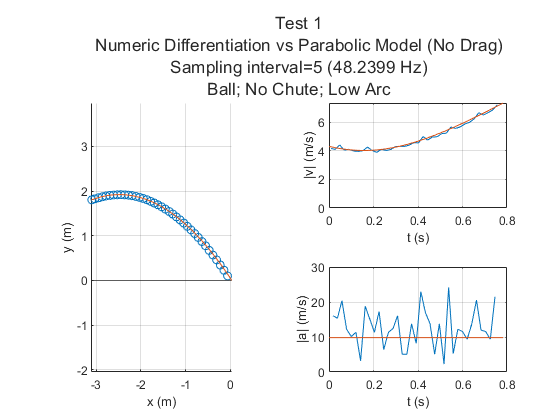
\includegraphics[width=0.9\linewidth]{images/Analysis1_Test1_Fig5_NoDrag.png}
\caption{\label{fig:Analysis1_Test1_Fig5_NoDrag} Fitting the parabolic model to sampled position data for a ball with no parachute. Left: Sampled position (blue) with the fit trajectory (orange). Right: Velocity and acceleration computed using numeric differentiation (blue) and the model's velocity and acceleration (orange). For low-drag scenarios, the parabolic model appears adequate.}
\end{figure}

So how does the parabolic model perform? We started by running it on some data of just the plain ball with no parachute attached, thrown in a low arc to minimize drag effects. This should be the best-case scenario for the parabolic model. The data is shown in Fig.~\ref{fig:Analysis1_Test1_Fig5_NoDrag}. 

At first glance, this model is actually looking pretty decent. There aren't any huge problems with the trajectory plot at this scale. Looking at the numeric differentiation, it's clear that there's plenty of noise in the signal. The velocity plot has some noise, and the model's velocity forms a smooth line through the middle of it. The noise in the signal makes the numeric differentiation's acceleration data useless, but the model's acceleration is a constant 1g as expected. If this projectile had been the only designed we cared about, we would probably just call it done here and saved ourselves a lot of work by not going straight to the linear drag model. 

%% Test 4

\begin{figure}[t]
\centering
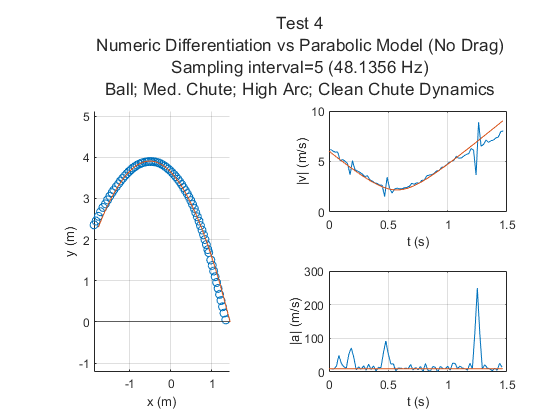
\includegraphics[width=0.9\linewidth]{images/Analysis1_Test4_Fig5_NoDrag.png}
\caption{\label{fig:Analysis1_Test4_Fig5_NoDrag} Fitting the parabolic model to sampled position data for a ball with a parachute. The parabolic model is unable to adequately capture the motion of this system.}
\end{figure}

\begin{figure}[t]
\centering
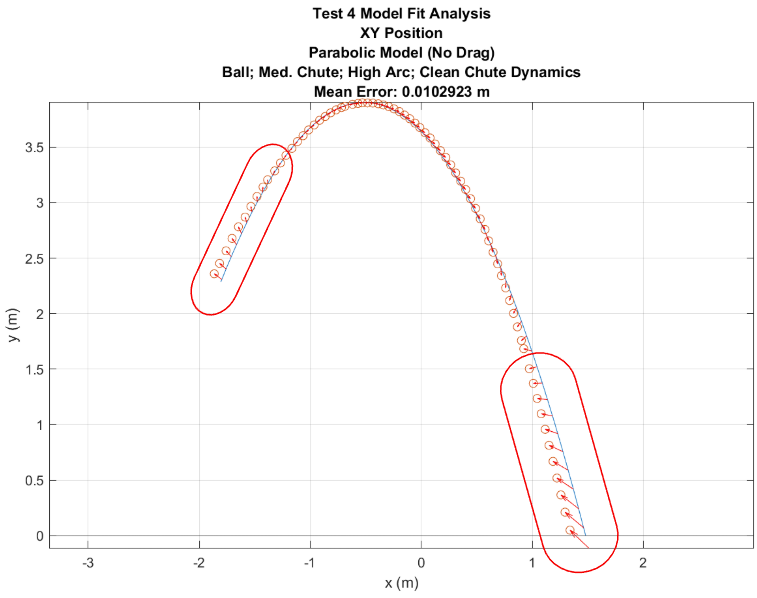
\includegraphics[width=0.9\linewidth]{images/Analysis1_Test4_Err_NoDrag.png}
\caption{\label{fig:Analysis1_Test4_Err_NoDrag} A closer look at the failure of the parabolic model. Red vectors show the error for each sampled position.}
\end{figure}

Next we tried a scenario with higher drag. Fig.~\ref{fig:Analysis1_Test4_Fig5_NoDrag} shows the results. 